Code reviewing has been a prevalent method of controlling code quality, detecting bugs, and increasing the understanding of the source code in the industry over the last five decades. It is a method that also yields learning and experience transfer between peers. This approach has become increasingly relevant in education to increase learning outcomes and the efficiency of project reviews, especially to prepare students for the working norms of the industry. \\

In industrial settings, the priorities for conducting code reviews often differ from those in educational contexts. In education, the main focus is on improving student learning and motivation. Therefore, it is important to streamline the review process to eliminate unnecessary steps and stages that are time consuming, tedious, and do not contribute enough value. A significant area for improvement is the selection of code files for review. During code reviews of larger projects, students do not need to evaluate the entire project; instead, focusing on the most relevant or crucial files can be more beneficial. By examining the impact and effect of code selection strategies, we can uncover valuable insights that can optimize the review process.


\section{Motivation and Problem Statement} \label{Motivation}
%The main objective of this research is to explore the efficiency of various methods in selecting code snippets and files for review in an educational context. This thesis aims to determine which selection techniques are useful for improving the review process, ultimately leading to improved learning outcomes for the reviewee and the reviewer. The goal will be to explore the methodologies behind the practice of code reviews in education. This research will support student learning and development by analyzing the process for conducting code reviews effectively. This is to ensure that students participating in code reviews are actively learning and honing their coding skills through the constructive feedback they exchange during peer reviews. \\

Code reviews are a vital activity in the software industry, where developers present their code to peers for inspection of defects, quality, and overall performance. This process improves code quality by detecting errors, bugs, and flaws, while also boosting project efficiency and facilitates knowledge sharing and collaboration among team members.~\cite{Bosu_Microsoft, Rigby_Bird_2013}. Such systematic reviews are crucial for maintaining high standards in software development. In educational contexts, this practice takes the form of peer reviews, a long-established and widely recognized best practice in academia. Here, peer review involves students evaluating each other's work, offering multiple benefits. These include providing timely feedback to the author and promoting learning opportunities for the reviewer~\cite{Indriasari_Luxton_2020}. Implementing this process allows students to actively engage in improving their own and their peers' work. \\

Integrating Peer Code Review (PCR) into higher education potentially combines the benefits of both traditional code reviews and peer reviews, introducing additional advantages. According to Indriasari et al.~\cite{Indriasari_Luxton_2020}, PCR enhances knowledge development, supports learning, improves code quality, improves review skills, streamlines processes for educators and provides social benefits. Moreover, Aalberg and Lorås note that active learning is a key component of PCR, enabling students to participate actively in their learning rather than passively receiving information~\cite{Aalberg_Lorås_2018}. This methodology not only prepares students for industry practices, but also equips them with the skills necessary to give and receive constructive feedback. While PCR and traditional code reviews offer various benefits, there remain significant opportunities for optimization, especially in educational contexts. Although the process successfully imports industry practices into academia, adapting them more effectively to meet educational needs and constraints can further improve their efficiency and impact. \\


To address the challenge of optimizing Peer Code Review processes in educational contexts, this thesis will perform a literature review and compare various different code selection techniques for the review process. This research will investigate existing studies and methodologies to determine how the efficiency of reviews can be improved. By examining articles and existing frameworks, the objective is to identify effective strategies that enhance the efficiency of the review process. Additionally, the motivations, advantages, and challenges associated with these methods in educational contexts will be investigated. Understanding these factors will offer a comprehensive perspective on how PCR and code reviews can be more effectively customized to meet educational requirements.


\section{Goal and Research Questions}
To address the motivations and problem described in Section 1.1, it is necessary to establish a goal and formulate research questions. These will guide the thesis and help resolve the various challenges.

\subsection{Goal}
As mentioned in Section \ref{Motivation}, the primary objective of this thesis is to improve the efficiency of Peer Code Review in educational contexts. This can be achieved by making the review process less time-consuming, more engaging, and hopefully, more effective in transferring knowledge. The focus of the thesis will be on optimizing the selection of code snippets and files to ensure that the time spent reviewing is more proportional to the knowledge gained and less draining on the motivation. The objective of this thesis is therefore to improve the productivity of the review process as well as the educational benefits. This will be achieved by identifying the most effective techniques for selecting crucial code for review.
\newpage

The specific goal to be addressed is:
\begin{quote}
    \textbf{\textit{Find the code selection techniques that are most effective in ensuring that the most critical code is selected for review in educational contexts, and investigate how these methods enhance the review process}}
\end{quote}

\subsection{Research Questions}

\noindent\textbf{RQ1:} How do code selection methods compare to each other?

- This question explores the practical impacts of different code selection techniques, focusing on their effectiveness in identifying and prioritizing critical code. Comparison of these techniques will reveal which methods are the most efficient and reliable, thus guiding best practices in reviewing code.\\


\noindent \textbf{RQ2:} How can code selection techniques be implemented in educational contexts?

- This question seeks to identify what challenges stand in the way of implementing code selection in the PCR process in educational contexts. Recognizing these obstacles makes it simpler to circumvent them in the future.\\


\noindent\textbf{RQ3:} What are the implications of different code selection techniques?

- This question investigates how various code selection techniques affect the learning experience, both the effectiveness, and their broader educational implications. Measuring how well these techniques identify and prioritize critical code will determine their overall utility and value in educational contexts.\\


\section{Research Approach}
In table \ref{tab:Research Approach}, the different phases of working with the thesis are presented. The research was carried out using a design-science research approach, which is explained further in Section \ref{Methodology}. \\

\begin{table}[H]
  \centering
  \begin{tabularx}{\textwidth}{>{\hsize=0.5\hsize}X >{\hsize=1.5\hsize}X}
    \textbf{Phases} & \textbf{Description} \\ [1ex] \hline 
    Planning & Define the scope, objectives, and timeline of the thesis. \\ [1ex]
    
    Literature review & Establish a solid foundation of existing knowledge and identify the gaps that my research will address. This helps define the problem description and the research questions. \\ [1ex] 
    
    Methodology & Outline the research methods to be used for selecting and analyzing the data. \\ [1ex]
    
    Selection methods & Research different methods and techniques for selecting relevant files. \\ [1ex]
    
    Implementation & Execute the research plan by collecting and processing the data using the selected methods. \\ [1ex]
    
    Data analysis & Analyze the data and compare the different methodologies. \\ [1ex]
    \\ \hline
    
  \end{tabularx}
  \caption{The different phases of working with the thesis}
  \label{tab:Research Approach}
\end{table}


\section{Contribution}
The contribution of this research is a detailed analysis of various code selection techniques used in Peer Code Reviews. This analysis systematically assesses and compares the effectiveness of these techniques in selecting critical code for review. The results indicate a notable variation in their effectiveness and applicability in educational contexts. This finding fills a gap in the current literature by providing a nuanced understanding of code selection techniques, and provides practical insights for their implementation in academic settings. \\

Furthermore, the thesis will conduct a review of existing literature to give a comprehensive look at the methodology of Peer Code Reviews. This perspective will improve academic understanding of how selecting specific code for review can influence the efficiency and effectiveness of educational Peer Code Reviews.


\section{Thesis Outline}
Table \ref{tab:Thesis Outline} presents the structure of the thesis, as well as the different chapters.

\begin{table}[H]
  \centering
  \begin{tabularx}{\textwidth}{>{\hsize=0.5\hsize}X >{\hsize=1.5\hsize}X} \hline
    \textbf{Chapter} & \textbf{Description} \\ [1ex]\hline 
    2 Background & Introduces the theoretical background and frameworks. A thorough literature review is performed. Some of the paragraphs in this chapter are rewritten sections from the previous work done in the preparatory project~\cite{Fordypningsprosjekt}. \\
    
    3 Methodology & An overview of the research method, context, procedure, analysis, and decisions. Presents how the experiment and comparisons will be performed. \\
    
    4 Results & Presents the results of the study. \\
    
    5 Conclusion & Discusses the results, contributions, future work, limitations, and findings of the thesis. \\
    \\ \hline
    
  \end{tabularx}
  \caption{Outline of the thesis structure}
  \label{tab:Thesis Outline}
\end{table}


\section{Sustainability}
The university has introduced requirements to reflect how the thesis relates to the United Nations' 17 Sustainable Development Goals (SDGs). This thesis aligns with SDG 4, which aims to provide quality education. It reads: 

\begin{quote}
\textbf{\textit{Ensure inclusive and equitable quality education and promote lifelong learning opportunities for all}}\cite{Nations}.
\end{quote}

By focusing on improving Peer Code Review processes in educational contexts, the research aims to improve the quality of education in informatics. The findings from the study promote more effective and engaging learning environments, allowing students to gain deeper insight and practical skills through collaborative learning and interaction. It equips students with critical skills essential for their professional development in the field of software engineering. Through these contributions, the research improves educational practices and prepares students to contribute effectively to the global knowledge economy, supporting the broader objectives of SDG 4.


\begin{figure}[H]
    \centering
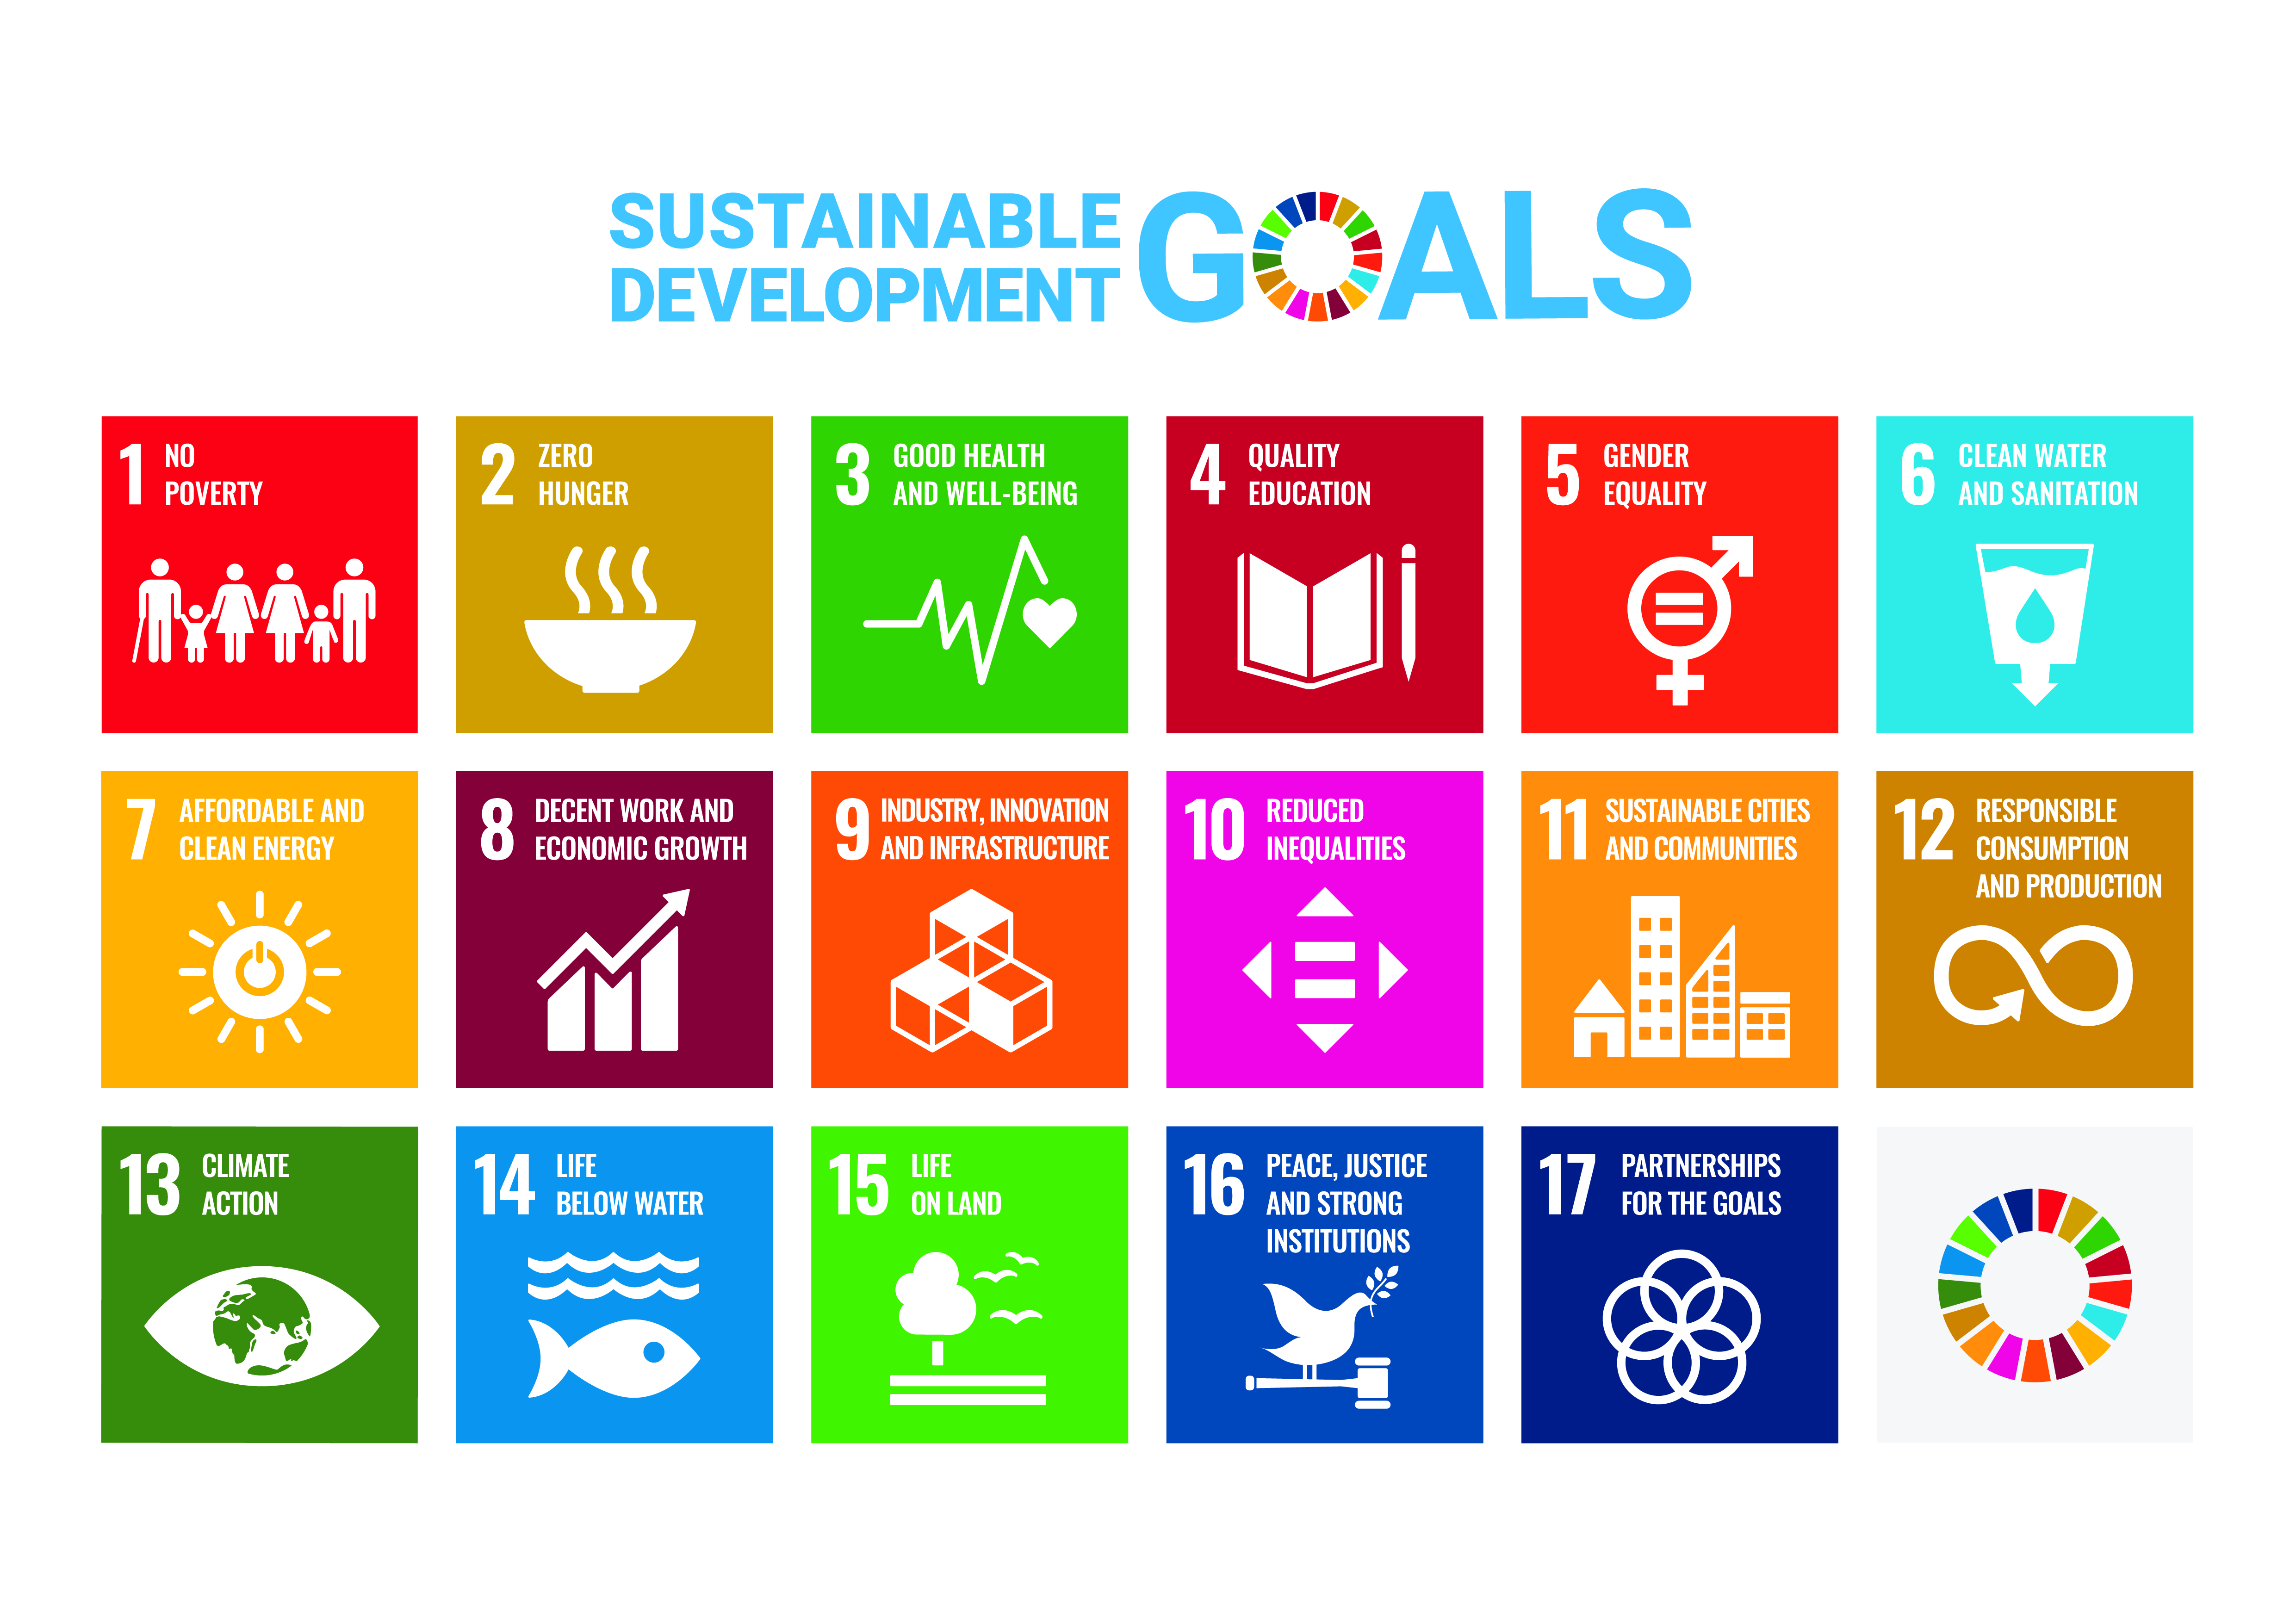
\includegraphics[width=0.65\textwidth]{Figures/SDG_2019.jpg}
    \caption{The UN's sustainable development goals~\cite{SDGs}}
    \label{fig:UN_SDGs}
\end{figure}